\documentclass[11pt]{article}
%Gummi|065|=)
\title{\textbf{Construir un amplificación con conexión Darlington}}
\author{Cabrera Gutiérrez Raúl\\
\textbf{ Matricula: 18312157}\\
Gutiérrez Olivares Rogelio\\
\textbf{Matricula: }\\
Sistemas Electrónicos de Interfaz\\}
\date{}
\usepackage{graphicx}
\begin{document}
\begin{figure}[htp]
\centering

\includegraphics[scale=3.00]{/home/raulcb/Downloads/ed3c.jpeg}
\caption{.}
\label{.}
\end{figure}
\maketitle

\section{Introducción}

En esta práctica se realizó una amplifición de señal, y con este poder activar un relevador. Este procedimiento fue realizado con dos trasnsistores comunes que juntamos en serie, esto paraamplificar la salida de señal y así poder activar el relevado que mas adelante,o como podriamos decír, la segunda parte se probó con un relevador de nivel industrial ya que este comunmente no trabaja con bajos voltajes sino altos.

\section{Objetivo}

Por medio de la utilización del transistor darlington activar un relevador industrial.
\section{Materiales}
\textbf{-Protoboard}
\textbf{-LDR}
\textbf{-Arduino}
\textbf{Transistor 2n2222a}
\textbf{-Relevador industrial 24v}
\textbf{-Diodo rectificador}
\textbf{Opto-acoplador 4n25}
\textbf{Resistencias varias}
\textbf{Potenciometro de 100k}
\textbf{Diodo emisor de luz}
\textbf{Relevador de 5vcc}

\section{Procedimiento}

Pra el procedimiento, fue necesario laprogramacion del arduino, ya que aqui van las entradas y las salidas las cuales nos ayudan para el funcionamiento.
\textbf{Armado}
\begin{figure}[htp]
\centering
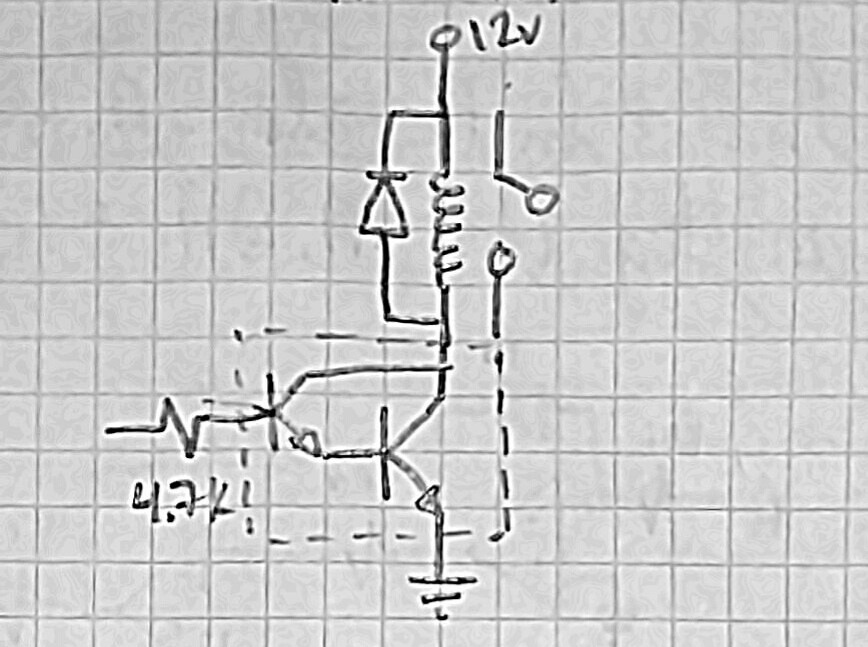
\includegraphics[scale=0.20]{/home/raulcb/Downloads/Darlington.jpeg}
\caption{.}
\label{.}
\end{figure}

Con este diagrama nos guiamos para armarlo ya que el diagrama nos muestra la forma de armarlo y conectar cada parte de los transistores correctamente.
En este caso como el transistor darlington no se consiguio optamos por poner dos transistores 2n2222a en serie y asi remplazar el darlington. 
El relevador industrial utiliza 24 v, por lo tanto necesitamos de uan fuente independiente ya poder accionar el relevador, ya que solo tenemos los 5v del arduino que no son los suficiente parapoder accionarlo.

\begin{figure}[htp]
\centering
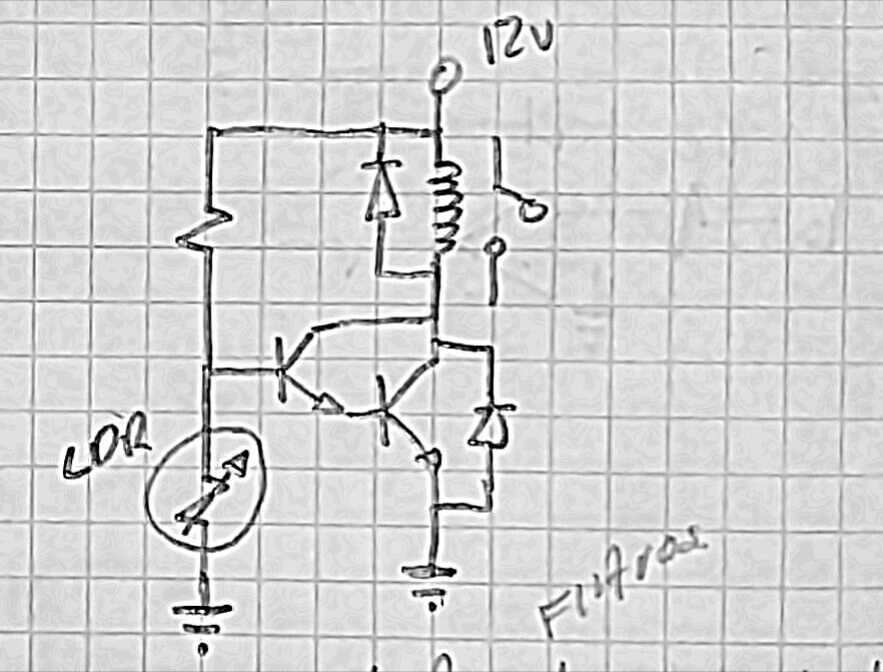
\includegraphics[scale=0.20]{/home/raulcb/Downloads/Dralington1.jpeg}
\caption{.}
\label{.}
\end{figure}

En este diagrama se muetra la primer parte utilizando un LDR. ESte componente varia su resistencia eléctrica dependiendo de la cantidad de luz que incide en él. Fotorresistor o fotorresistenci.  
En este caso es similar a la parte del relevador industrial
El LDR es una parte importante, ya que cuando la luz es obstruida en esta fotorresistencia activara una mayor potencia, y así activar el relevador, esta conexion donde va la parte del relevador es la msima, pero en este caso solo sustituira la interfaz de entrada. 

\section{Resusltado}
\begin{figure}[htp]
\centering
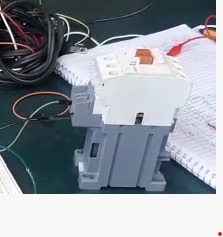
\includegraphics[scale=0.60]{/home/raulcb/Downloads/Reley ind.jpeg}
\caption{..}
\label{..}
\end{figure}
El relevador industrial activa su pata caundo se presiona el push botton.
\begin{figure}[htp]
\centering
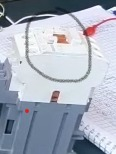
\includegraphics[scale=0.50]{/home/raulcb/Downloads/activa.jpeg}
\caption{.}
\label{.}
\end{figure}
Sube y baja esta parte, así nos damos cuenta de que se esta activando. Pero ne la parte del LDR, solo en el momento en el que tapamos la luz esteaumenta su potencia y permite el relevador se encienda y para poder saber como es que funciona, tiene un cliqueo al momento de accionar.
\begin{figure}[htp]
\centering
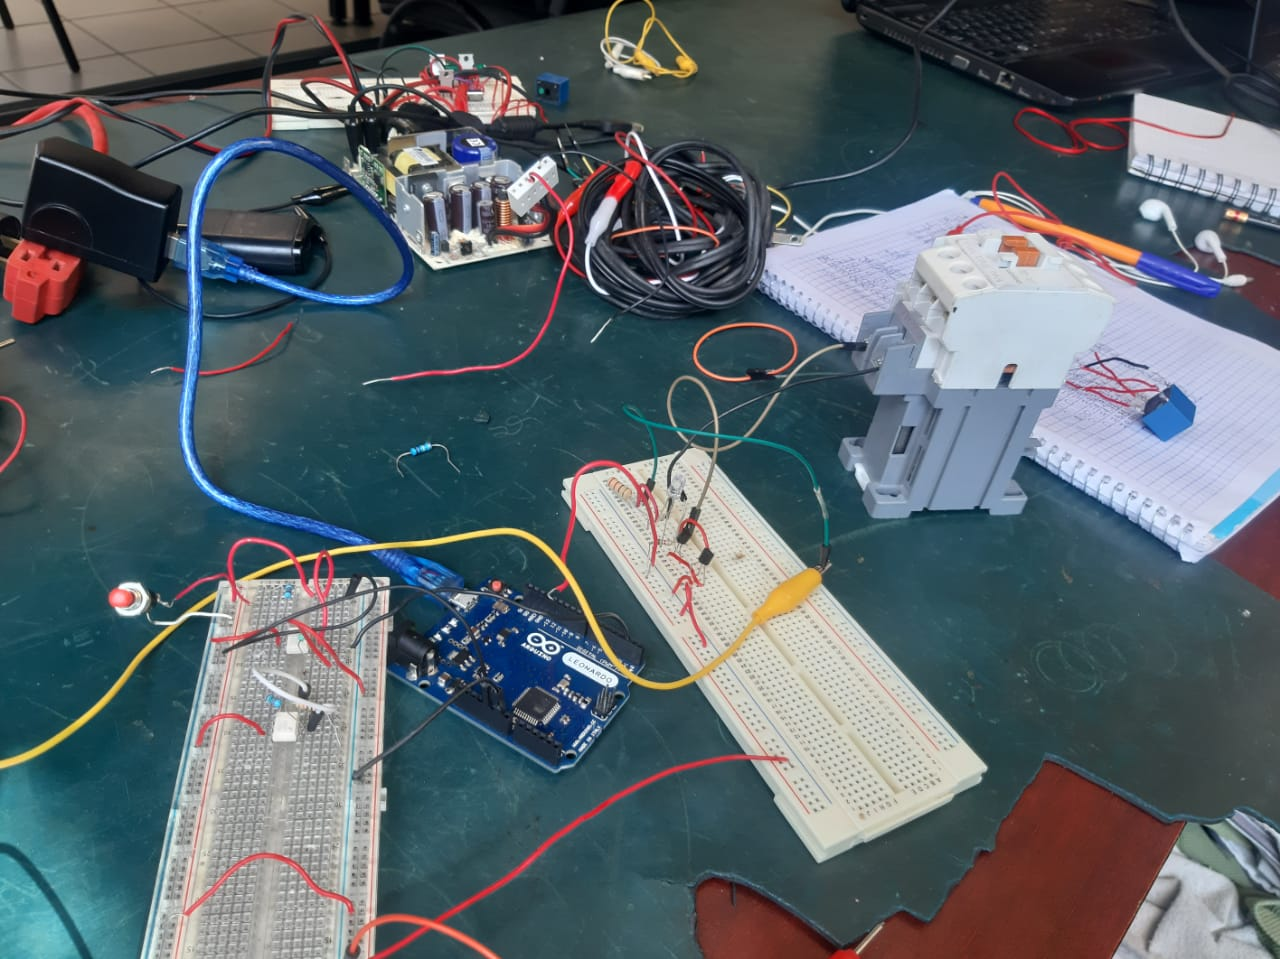
\includegraphics[scale=0.20]{/home/raulcb/Downloads/LDR.jpeg}
\caption{.}
\label{.}
\end{figure}
Podemos ver todo el circuito con las dos pates, una con LDR y el otro con el relevador industrial.
\section{Conclusón}
El amplificador Darlington aplicado en un circuito genera una gran funcionalidad la cual aporta un gran conocimiento total a lo ya visto antes, lo que lo vuelve importante para nuestros estudios y lo que resta dentro de la carrera y a su vez el poder incluirse en trabajos posteriores a la materia que  ayudara a darles una mayor plusvalía la cual mejorara nuestro perfil de trabajo y la estética estructuras de nuestros proyectos dentro de nuestra vida profesional.
 Podemos ver en estas prácticas el funcionamiento de estos componentes y entender en que otras áreas o en que dispositivos podemos encontrar estos usos, así darnos cuenta lo fácil o sencillo que es esto.


\end{document}
